%%%%%%%%%%%%%%%%%%%%%%%%%%%%%%%%%%%%%%%%%%%%%%%%%%%%%%%%%%%%%%%%%%%%%%%%%
\subsection{Motivation:  spatial locality in KV-storage}
% KV-storage workloads} 
%%%%%%%%%%%%%%%%%%%%%%%%%%%%%%%%%%%%%%%%%%%%%%%%%%%%%%%%%%%%%%%%%%%%%%%%%

% KV-stores are everywhere
Key-value stores (KV-stores) are widely used  by a broad range of applications and are projected
to continue to increase in popularity in years to come; market research  identifies them as the 
``driving factors'' of the NoSQL market, which is expected to garner \$4.2B by 2020~\cite{alliedmarketresearch}.

% In many applications, keys are composite
KV-stores provide a simple programming model. 
Data is an ordered collection of key-value pairs, and the API supports random writes, 
random reads, and range queries. 

A common design pattern is the use of \emph{composite} keys that represent an agglomerate of attributes.
Typically, the first attribute -- called the \emph{primary key} -- has a skewed distribution, and so   access via the composite key exhibits \emph{spatial locality}, as 
popular primary keys result in popular \emph{key ranges}. 

One example of this arises in mobile analytics platforms, e.g., AppsFlyer~\cite{appsflyer}, Flurry~\cite{flurry}, 
and Google Firebase~\cite{firebase}. %~\cite{medium-mobile-analytics}.   
Such platforms %help mobile developers collect user activity data, analyze it, and optimize their app experience. They 
ingest massive streams of app event reports %(e.g., start, stop, or particular scenario within an app), 
in  real-time and provide a variety of insight queries into the data. For example, Flurry provided insights for  
1M+ apps across 2.6B user devices  in 2017~\cite{FlurryReport2017}. In order to offer per-app analytics efficiently,
such services aggregate data in KV-stores indexed by a composite key prefixed by a unique app 
id,  followed by a variety of other attributes (time, user id, device model, location, event type, etc.).
%
We examine a trace of $200$ million events captured from a production mobile analytics engine over the course of four minutes.  
\Cref{fig:cdf} shows the access frequency distribution over the  $40$K app ids occurring in this stream. It follows a marked
heavy-tail pattern: $10$\% of the apps cover over $99.5$\% of the events; $1$\% of them  cover $94$\%; and fewer 
than $0.1$\% cover $70$\% of the events. 

% This means the data is highly skewed and with a very long tail (not depicted in the figure).
%Table~\ref {table:popular} shows the cumulative probability of the top-$20$ popular applications, covering more than $50$\% of the events. 
%With application name as the primary dimension of a composite key this distribution induces high spatial locality.


\begin{figure}[tb]
\centering
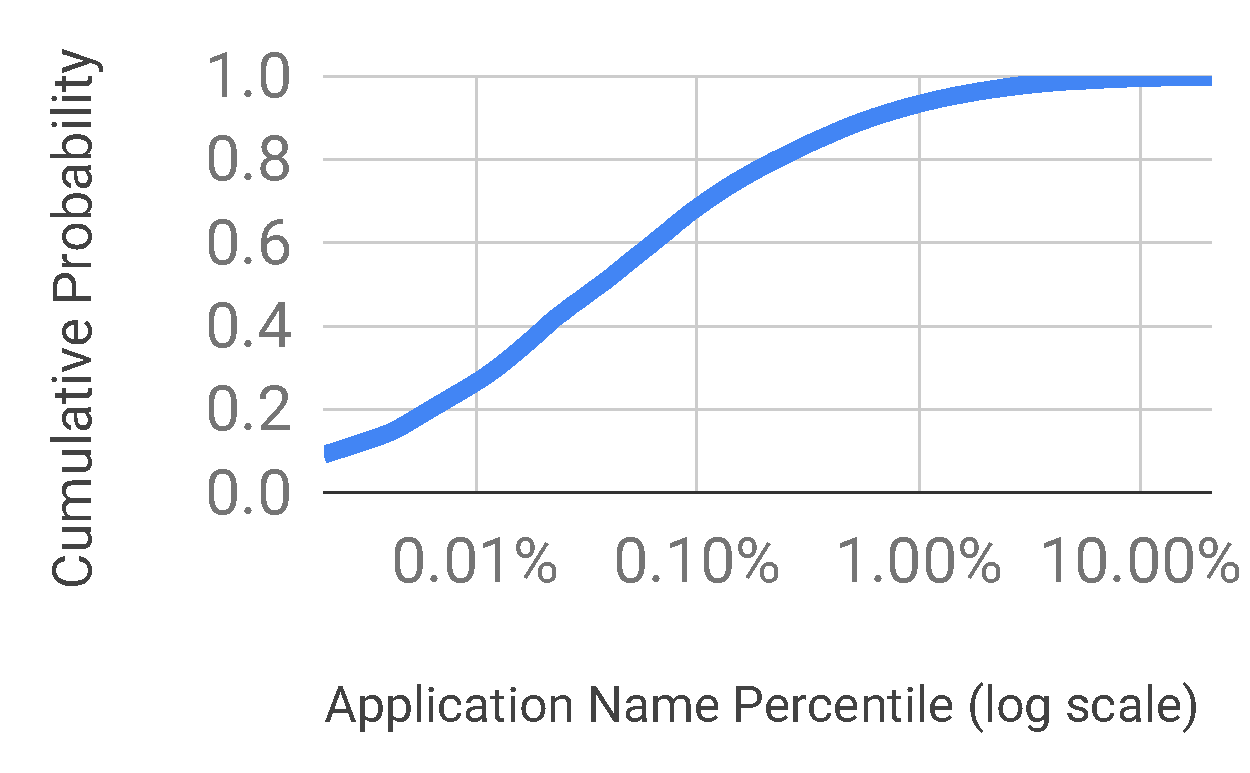
\includegraphics[width=0.6\columnwidth]{figs/cdf.pdf}
\caption{CDF of app ids in a real-world mobile analytics event stream consisting of 200 million events. \inred{Name -> id}}
\label{fig:cdf}
\end{figure}

Composite keys arise in many additional domains, including messaging and social networks. 
For example, a backend Facebook Messenger query may retrieve the last 100 messages for a 
given user~\cite{Borthakur:2011:AHG:1989323.1989438}; %, where the primary key is user id. 
in Facebook's social network, a graph edge is indexed by a key consisting of two 
object ids and an association type~\cite{Armstrong:2013:LDB:2463676.2465296}.
%Note further that 
Spatial locality   also arises with simple (non-composite) keys, for example, when 
reverse  URL domains are used as keys for web  indexing~\cite{Cho:1998:ECT:297805.297835}. 

% Overfitting for Zipf 
The prevalence of skewed (e.g., Zipfian)  access  in real workloads is widely-recognized 
and reflected in standard benchmarks (e.g., YCSB~\cite{YCSB}). %  feature heavy-tailed key-access distributions like Zipf.
But these benchmarks fail to capture the spatial aspect of locality.
This, in turn, leads to storage systems being optimized for a skewed distribution on individual keys, % with no spatial locality,
e.g., in partitioning data by  recent access time as opposed to by key range.
In this work, we make spatial locality a first-class consideration in KV-store design.
% which leads us to rethink the design principles underlying today's popular KV-stores.



%%%%%%%%%%%%%%%%%%%%%%%%%%%%%%%%%%%%%%%%%%%%%%%%%%%%%%%%%%%%%%%%%%%%%%%%%
\subsection{Spatial locality: the challenge }  
%%%%%%%%%%%%%%%%%%%%%%%%%%%%%%%%%%%%%%%%%%%%%%%%%%%%%%%%%%%%%%%%%%%%%%%%%



% LSM is the standard 
The de facto standard design for high-throughput KV-stores today is \emph{LSM} (log-structured merge) trees~\cite{DBLP:journals/acta/ONeilCGO96}. 
LSMs initially group writes  into files \emph{temporally}, and not by key-range. 
A background \emph{compaction} process later merge-sorts any number of files, grouping data by keys. 

% LSM is  not ideal for spatial locality  because of  temporal grouping 
This approach is not ideal for workloads with high spatial locality for two reasons. 
First,  popular key ranges are fragmented across many files. 
Second,  compaction  is costly in terms of  both performance 
(disk bandwidth) and \emph{write amplification}, namely the number of physical writes 
associated with a single application write. The latter is  particularly important in SSDs as it increases disk wear. 
The temporal grouping means that compaction is indiscriminate with respect to key popularity:  
Since new (lower level) files are always merged with old (higher level) ones, 
 ``cold'' key ranges  continue to be repeatedly re-located by  compactions.  

% LSM is not the best when the entire working set fits in memory
Another shortcoming of LSM is that its temporal organization, while optimizing disk I/O,  penalizes in-memory operation. 
All updates -- including ones of popular keys -- are flushed to disk, even though persistence is assured via a separate \emph{write-ahead-log (WAL)}.
Beyond increasing write amplification, this makes the flushed keys unavailable for fast read from memory,
which is  wasteful if the system incorporates sufficient DRAM to hold most of the active working set. 
The drop in DRAM prices (more than $6.6$x since 2010~\cite{dram-prices}) makes the latter scenario increasingly common.  

Yet  LSMs have supplanted the  traditional spatial data partitioning of B-trees for a reason~\cite{rocks-vs-inno}.
%A crucial challenge arising in spatially-organized  storage is how to persist all updates in a consistent way without sacrificing performance.
In  B-trees, each update induces random I/O  to a leaf, resulting in poor write performance.
Moreover, the need to preserve a consistent image of a leaf while it is being over-written induces high write amplification. 
$B^{\epsilon}$-trees~\cite{Brodal:2003:LBE:644108.644201} mitigate this cost using write buffers. % in internal tree nodes. 
However, this slows down lookups, which now have to search in unordered buffers, possibly on disk. 
% If the buffers reside on disk, the lookup time is unacceptably slow, whereas if they are in RAM then they have to be complemented by a separate persistence mechanism, with its own costs.  
%
LSMs, in contrast, achieve high write throughput by absorbing  writes in memory and periodically flushing them as 
sequential files to disk; they expedite reads by caching data in DRAM.

The resounding performance advantage of the LSM approach over B- and B$^{\epsilon}$-trees has been repeatedly demonstrated, 
e.g., in a recent  study of the Percona mySQL server using three storage engines -- RocksDB, TokuDB, and InnoDB --
based on LSM, a B$^{\epsilon}$-tree, and a B-tree, respectively~\cite{toku-rocks-inno}.
%
Another advantage of LSMs is ensuring consistency -- in particular, atomic scans --   under multi-threaded access. 
%This can be  tricky when a scan spans both memory-resident and disk-resident data.
LSMs provide atomic scans without locks using multi-versioning. 
In contrast, databases based on B- or  B$^\epsilon$-trees either use locks~\cite{innodblocking} 
or forgo scan consistency~\cite{tucana}.



\remove{
Obviously, we do not claim that spatial data partitioning is new; indeed, classical B-trees~\cite{DBLP:conf/sigmod/BayerM70,Comer79} 
 pre-date  LSM trees, and many B-tree variants~\cite{Brodal:2003:LBE:644108.644201,Bender15, Lehman:1981:ELC:319628.319663} have  emerged over the years. 
 However, it is important to note that these trees are  conceptual constructs rather than storage systems; 
 employing these concepts within a practical data store over a memory hierarchy 
 raises multiple challenges,  which perhaps explains their limited adoption in industrial KV-stores.
 A key challenge is what to persist when and in what format. 
 }
 
Our  goal is to 
%draw attention to the importance of spatial locality in today's KV-store workloads and to 
put forth a KV-store design alternative  suited for the 
spatial locality arising in today's  workloads, without forfeiting the benefits achieved by the LSM approach.


%We are not aware of any published solution for atomic scans in storage based on  B- or  B$^\epsilon$-trees.

%%%%%%%%%%%%%%%%%%%%%%%%%%%%%%%%%%%%%%%%%%%%%%%%%%%%%%%%%%%%%%%%%%%%%%%%%
\subsection{Our contribution: \sys}
%%%%%%%%%%%%%%%%%%%%%%%%%%%%%%%%%%%%%%%%%%%%%%%%%%%%%%%%%%%%%%%%%%%%%%%%%

% Drum roll 
We present \sys, a high-throughput persistent KV-store geared towards spatial locality. 
\sys's  architecture (\cref{sec:principles}) combines a spatial data organization with LSM-like  batch I/O. 
The pillars of our design are large \emph{chunks} holding contiguous key ranges. 
\sys's chunks are not merely  a means to organize data on-disk (like nodes in a B-Tree); they 
are also the basic units for DRAM caching, I/O-batching, logging, and compaction. 
This approach is unique:  typical storage systems rely on OS-managed page caches (whereas chunks consist of many pages),  
supplemented by application-level caches of individual rows (KV-pairs) that serve only the read-path; 
they use WALs for the write-path.

Our novel chunk-based organization has several benefits. 
First, chunk caching is effective for spatially-local workloads.
Second, chunk-level logging eliminates the need to log each update in a dedicated WAL, thus 
reducing write amplification and expediting crash-recovery. 
Finally, using the same data structure for both the read-path (as a cache) and the write-path
(as a log) allows us to perform \emph{in-memory compaction}, reducing write amplification even further.

% Downsides
The downside of spatial partitioning is that if the data lacks spatial locality and the active working set is big, 
caching an entire chunk for a single popular key is wasteful. 
We mitigate this by adding a \emph{row cache} for read access to hot keys. Even so, 
our design is less optimal for mixed read/write workloads lacking spatial locality, for which the LSM approach may yield better performance.  

%To further expedite access in different scenarios, we incorporate a number of additional mechanisms: 
%a volatile index for direct access to chunks by key; Bloom filters to reduce reads from disk-resident chunks; and 

Our algorithm (\cref{sec:design}) is designed for high concurrency. 
%among threads running put, get, and scan operations, as well as background maintenance (compaction). 
It supports atomic scans using low-overhead multi-versioning, where versions are increased only by scans and not by updates. 
It ensures consistency and correct failure-recovery. 
%While the mechanisms we employ are all variants of ones appearing in the literature, their combination is novel and results in a high-performance storage system.

We implement \sys\ in  C++ (\cref{sec:impl}) and extensively evaluate it (\cref{sec:eval})
via three types of workloads: (1) a production trace collected from a large-scale mobile analytics platform; 
(2)  workloads with synthetically-generated composite keys exercising  standard YCSB scenarios~\cite{YCSB};
and (3)  YCSB's traditional benchmarks, which employ simple (non-composite) keys.  
%In all cases, 
We compare \sys\ to the recent (Oct 2018) release of RocksDB~\cite{RocksDB}, a mature industry-leading LSM KV-store. 
We  experimented with two additional open-source KV-stores, PebblesDB~\cite{PebblesDB} (a recent LSM KV-store) and  
% PreconaFT/
TokuDB~\cite{TokuDB} (the only publicly-available $B^{\epsilon}$-tree-based 
KV-store); both performed significantly worse than  RocksDB and \sys, so we focus on RocksDB results. 
%so we do not discuss them further.
%\inred{across the entire YCSB benchmark suite.} %, which is in line with previous studies of PerconaFT~\cite{tucana}, so we excluded them from further tests. 
Our main findings are: 
\begin{enumerate} 
  %   \setlength{\itemindent}{-10pt}
\item \sys\/ is dramatically better under high spatial  locality.  
For instance, on a 256GB production dataset, \sys\ ingests data 3.7x faster than RocksDB %,  scans recent  data up to 27\% faster, 
and reduces write amplification by almost 4x. 
%And in large synthetic composite-key workloads, \sys\  improves over RocksDB's throughput by $24\% - 75\%$. 
\item \sys\/ significantly outperforms RocksDB whenever most of the working set fits in RAM, 
%For example, with synthetic composite keys and a memory-resident working set, \sys\  
accelerating scans by up to $3.5$x, puts by up to $2.3$x, and gets by up to $2$x. 
\item \sys's performance is  comparable to RocksDB's in traditional YCSB workloads without spatial locality.
%while its write amplification is much smaller.
\item RocksDB outperforms \sys\ (by 20--25\%)  in mixed read/write workloads with large active working sets and no spatial locality, 
although \sys's write amplification remains $\sim$2x smaller than RocksDB's. 
%\item \sys\ has lower write amplification, especially on large datasets.
\end{enumerate}

% Benefits
Our results underscore the advantage of \sys's spatially-organized chunks:
(1) little fragmentation of key ranges  yields better  performance under spatial locality; 
(2) keeping hot ranges in memory leads to better performance when most of the working set fits in RAM; and 
(3) in-memory chunk compaction saves disk flushes and reduces write volume.  
In addition, in-chunk WALs  allow quick recovery from crashes with no need to replay any WAL.


~\cref{sec:related}  surveys related work and~\cref{sec:conclusions} concludes this paper. 
